\documentclass[12pt]{article}

% Layout.
\usepackage[top=1in, bottom=0.75in, left=1in, right=1in, headheight=1in, headsep=6pt]{geometry}

% Fonts.
\usepackage{mathptmx}
\usepackage[scaled=0.86]{helvet}
\renewcommand{\emph}[1]{\textsf{\textbf{#1}}}

\usepackage[group-separator={,}]{siunitx}

% TiKZ.
\usepackage{tikz, pgfplots}
\usetikzlibrary{calc}
\usetikzlibrary{calc,trees,positioning,arrows,fit,shapes,through, backgrounds}
\usetikzlibrary{patterns}

\usetikzlibrary{decorations.markings}
\usetikzlibrary{arrows}

\usepackage{pgfplots}

\usepackage{longtable}
\usepackage{tabularx}


% Misc packages.
\usepackage{amsmath,amssymb,latexsym}
\usepackage{graphicx}
\usepackage{array}
\usepackage{xcolor,enumerate, tabularx,adjustbox}
\usepackage{multicol}
\usepackage{fancyhdr}
\pagestyle{fancy}


% Misc.
\renewcommand{\d}{\displaystyle}
\newcommand{\ds}{\displaystyle}
\newcommand{\ul}[1]{\underline{#1}}
\def\bc{\begin{center}}
\def\ec{\end{center}}
\def\be{\begin{enumerate}}
\def\ee{\end{enumerate}}

\newcommand{\ans}[1][1in]{\rule{#1}{.5pt}}


\lhead{Exam III Review}
\rhead{}

\begin{document}

%\noindent{\Large{Summary of Topics}}
\section*{Summary of Topics}
\begin{enumerate}
\item Scheduling
\begin{itemize}
\item Know how to construct a digraph from a dependency list
\item Know the meaning of the following
\be
\item Project digraph
\item schedule
\item priority list
\item processor
\item critical path
\item critical time
\item idle time
\item decreasing time algorithm/priority list
\item backflow algorithm
\item critical time priority list
\ee
\item Be able to create a schedule from a digraph or table of dependencies and a priority list, and determine the finishing time, idle time, and whether the schedule is optimal
\end{itemize}
\item Cryptography
	\begin{itemize}
	\item Know how to encrypt and decrypt a message using
		\begin{itemize}
		\item a Caesar cipher
		\item an alpha-numeric cipher given a substitution mapping
		\item a transposition cipher given the length of a row
		\item a transposition cipher given an encryption keyword
		\item a shifting substitution / progressive Caesar cipher
		\item a Vigen\`{e}re cipher
		\item a double transposition cipher (given two keywords)
		\end{itemize}
	\item Know how to use letter frequency to decrypt a message without an encryption key.
	\item Know which encryption methods do or do not preserve letter frequency.
	\item Be able to articulate strengths and weakness in each of the encryption methods learned.
	\item Be able to recognize and explain why some keywords are good and some are not.
	\end{itemize}		
\end{enumerate}

\subsection*{\Large{Tabula Recta}}

A Tabula Recta is provided on the last page. It will be provided on the exam as well.

\newpage
%\begin{center} {\Large{Scheduling}} \end{center}
\section*{Scheduling Sample Problems}
\begin{enumerate}
\item The table below contains the tasks to be completed for a project.

\begin{tabular}{| c|c|c|}
\hline
task& time& dependencies/\\
&(in minutes)&prerequisites\\
\hline
A&2&\\ \hline
B&9&\\ \hline
C&3&\\ \hline
D&7&A\\ \hline
E&1&C\\ \hline
F&6&A\\ \hline
G&4&E\\ \hline
H&8&D,F\\ \hline
I&5&G\\ \hline
J&1&B,H,I\\ \hline
\end{tabular}
	\begin{enumerate}
	\item Next to the table, create a \emph{digraph} representing the project.
	\item Find a \emph{critical path} and its corresponding \emph{critical time}. Explain the significance of the critical time.
	\vfill
	\item Create a priority list using the \emph{decreasing time} algorithm. (That is, create a priority list ordered by decreasing time.)
	\vfill
	\item Use the \emph{Backflow algorithm} to assign critical numbers to each vertex in the graph above.
	\item Create a priority list using the critical time algorithm. (That is, create a priority list ordered by decreasing \emph{critical} time.)
	\vfill
	\item How long would it take for one processor to complete all the tasks? \ans
	\vfill
	\item Is it possible for 2 processors to complete a schedule in exactly the critical time?  Why or why not? Provide a supporting calculation.
	\vfill
	\end{enumerate} 
\newpage
\item Use the diagraph below and the given priority list to construct a schedule using two processors.

\def\r{2}
\def\s{.6}

\begin{tikzpicture}[vtx/.style={draw, circle, inner sep = 3pt, font = \scriptsize}, myto/.style={-latex, shorten >=2pt, shorten <=2pt
}, node distance = \r cm]
\node[vtx, label=above:{\scriptsize $A(10)$}, ] (A) at (0,0){};
\node[vtx, below = \s cm of A, label=above:{\scriptsize $B(5)$}] (B) {};
\node[vtx, below =\s cm of B, label=above:{\scriptsize $F(3)$}] (F) {};
\node[vtx, right = of B, label=above:{\scriptsize $C(4)$}] (C) {};
\node[vtx, right = 2*\r of C, label=above left:{\scriptsize $D(1)$}] (D) {};
\node[vtx, right =of D, label= right:{\scriptsize $E(8)$}] (E) {};
\node[vtx, right = of F, label=below:{\scriptsize $G(1)$}] (G) {};
\node[vtx, right =of G, label=below:{\scriptsize $H(7)$}] (H) {};
\node[vtx, below =\s cm of H, label=below:{\scriptsize $J(6)$}] (J) {};

\foreach \i/\j in {B/C,F/C,F/G,G/H,G/J,C/D,D/E, H/D}{\draw[myto] (\i) -- (\j);}
\end{tikzpicture}

Construct a schedule using the priority list \[F,\ B, \ G,\  C, \ A, \ H,\  J,\  D,\ E\]

\hspace*{-1in}	\begin{tabular}{c || c}
time &   \quad \hspace{6in} \quad \\ \hline
ready& \\ \hline
done& \\ \hline
\end{tabular}

\hspace*{-1.5cm}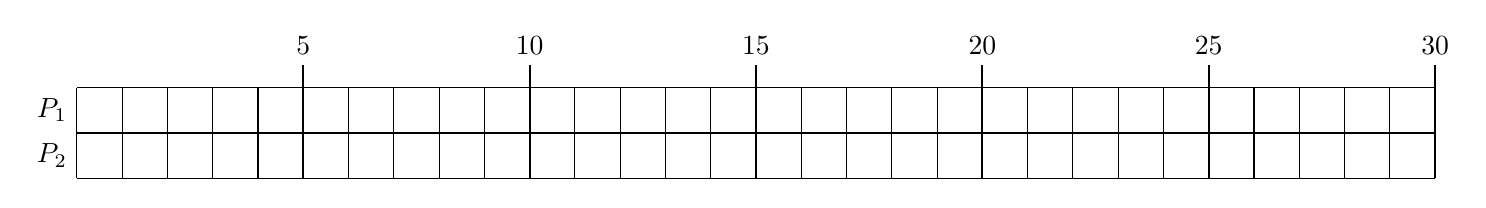
\begin{tikzpicture}[scale = 1.15, lbl/.style={font=\tiny, inner sep = 1 pt, fill = white}]
\path (0, 3/4) node[left] {$P_{1}$};
\path (0, 1/4) node[left] {$P_{2}$};
\draw[step=1/2] (0,0) grid (30/2, 2/2);
\foreach \i in {5, 10, ..., 30}{\draw[thick] (\i/2,0) -- (\i/2,2/2+1/4) node[above]{\i};}
\end{tikzpicture}

Finishing time: \ans

Idle time: \ans

Critical path / time: \hrulefill

Is your schedule optimal? How do you know?

\vfill

 
\end{enumerate}

\bigskip

%%Page 1

%\textbf{Formulas}\\
%$$ A=P+I \quad \hspace{1cm} \quad A=P(1+rt) \quad \hspace{1cm} \quad A=P\left(1+\frac{r}{n}\right)^{(nt)} \quad \hspace{1cm} \quad P=\frac{A}{\left( 1+\frac{r}{n}\right)^{(nt)}} $$
%
%$$ P=\frac{d(1-\left(1+\frac{r}{n}\right)^{(-nt)}}{\left(\frac{r}{n} \right)} \hspace{1cm} \quad d= \frac{P\left(\frac{r}{n} \right)}{\left( 1- \left(1+\frac{r}{n}\right)^{(-nt)}\right)}$$
%	\begin{itemize}
%	\item Calculate tip on a bill.
%	\item Know the terminology and notation of principal ($P$), interest ($I$), annual interest rate ($r$), compounding frequency ($n$), time ($t$), payment amount ($d$), and future value ($A$).
%	\item Be able to identify those variables given a finance formula.
%	\item Distinguish between simple interest and compound interest.
%	\item Distinguish between an annual interest rate (APR) compounded at some rate and the effective annual interest rate (EAR).
%	\item Know how to calculate (which formula to use) the future value, $A$, and interest, $I,$ over a period of years $t$ in a savings account or loan given an annual rate $r$, in the case where the interest is simple or compounded at a given number of periods $n$ per year.
%	\item Know how to calculate (which formula to use) the principal, $P,$ required to obtain a given future value on a savings or loan account given the time period, annual interest rate and compounding rate.
%	\item Know how to calculate (which formula to use) the monthly payment on a loan of a given amount at a given rate and time and then the total amount paid for the loan.
%	\end{itemize}
%\end{enumerate}
%\newpage
%page 2
\newpage
\section*{Cryptography Sample Problems}
%\noindent{\Large{Sample Problems}}
\begin{enumerate}
\item Encrypt the message GO TO BERLIN using
	\begin{enumerate}
	\item a Caesar cipher with a shift of 24 (A $\to$ Y)
	\vspace{1in}
		\item a transposition cipher given a row length of 5.
	\vfill
	\item a transposition cipher given encryption keyword {\tt STOP}.
	\vfill

	\item a shifting substitution cipher (progressive Caesar cipher) starting with a shift of 6 (A to G).
	\vfill
		\newpage
	\item a Vigen\'{e}re cipher with key word {\tt STOP}.
	\vspace{1in}
	\item a double transposition cipher with first key word {\tt BLUE} and second key word {\tt GOLD}.
	\vfill
	\end{enumerate}
\item Using the alpha-numeric substitution below to answer the questions.

{\small
\begin{tabular}{|c|c|c|c|c|c|c|c|c|c|c|c|c|c|c|c|c|c|c|}
\hline
%&0&1&2&3&4&5&6&7&8&9&10&11&12&13&14&15&16&17\\ \hline \hline
original& A&B&C&D&E&F&G&H&I&J&K&L&M&N&O&P&Q&R\\  \hline
maps to&9&8&7&6&5&4&3&2&1&0&D&C&B&A&H&G&F&E\\
\hline
\end{tabular}

\begin{tabular}{|c|c|c|c|c|c|c|c|c|c|c|c|c|c|c|c|c|c|c|}
 \hline
%&18&19&20&21&22&23&24&25&26&27&28&29&30&31&32&33&34&35\\ \hline \hline
original &S&T&U&V&W&X&Y&Z&0&1&2&3&4&5&6&7&8&9\\ \hline
maps to&L&K&J&I&P&O&N&M&T&S&Q&R&V&U&Y&X&W&Z \\
%[12pt]
\hline
\end{tabular}
}

	\begin{enumerate}
	\item Encrypt the plaintext: RIGHT 10 LEFT 25
	\vspace{1in}
	\item Decrypt the ciphertext: \quad K5OKT \ \  TQXW
	\vspace{1in}
	\end{enumerate}
\newpage
\item Decrypt each encrypted text using the specified mechanism.
	\begin{enumerate}
	\item ciphertext: NJCYQC \\encryption mechanism: a Caesar cipher with a shift of 24 (A to Y)
	\vspace{1in}
	\item ciphertext: DFTOO \;\: ANRBO \;\: GCTED \\encryption mechanism: a transposition cipher given a row length of 5
	\vfill
	\item ciphertext: DMFAT \:\: 3RYME \:\: IIIRS \:\: D \\ encryption mechanism: a transposition cipher given encryption keyword STOP
	\vfill
	\item ciphertext: HYQWQ \\encryption mechanism: a shifting substitution cipher / progressive Caesar cipher starting with a shift of 6 (A to G)
	\vfill
	\newpage
	\item cipher text: FHHTK \:\: ASTL \\encryption mechanism: a Vigen\`{e}re cipher with key word {\tt STOP}
	\vfill
	\item cipher text: OEAOM \:\: NTSLD \\encryption mechanism: a double transposition cipher with first key word {\tt BLUE} and second key word {\tt GOLD}.
	\vfill
	\vfill
	\end{enumerate}
\item Which of the encryption methods in problems 1 and 2 above preserve letter frequency?
\vfill

\newpage
%\newpage
%\item Pikachu takes out a \emph{simple interest} loan of \$500 with an annual interest rate of 6.24\%. Suppose Pikachu repays the loan in 2 years and 4 months later.
%	\begin{enumerate}
%	\item How much did Pikachu pay? Write down what calculation you are doing, and provide a numeric answer.
%	\vfill
%	\item How much of the payment was interest? Write down what calculation you are doing, and provide a numeric answer.
%	\vfill
%	\end{enumerate}
%	
%	
%For the next two problems, 
%%\item Among the parameters $P$, $A$, $I$, $n$, $t$, $d$, $r$, which values are given to you in the problem?
%\emph{write down a calculation} (plug in numbers) you would need to put into a spreadsheet or calculator to answer the problem.
%You do not need to actually determine the numerical answer (although you're welcome to do so for this review). 
%
%
%	
%\item Charizard invests in a certificate of deposit that offers 4.2\% APR compounded daily.
%
%
% 
%	\begin{enumerate}
%	\item If Charizard invests \$1000, how much will be in the account in 10 years? (We are supposing no additional investments or withdrawals over the 10 years.)
%	\vfill
%	\item How would you compute the effective annual interest rate (EAR) of this investment?\vfill
%	\item How much would Charizard need to invest in order for the account to contain \$10,000 at the end of 20 years?
%	\vfill
%	\end{enumerate}	
%	
%	\newpage
%	
%\item Mewtwo takes out a 15 year mortgage for \$150,000 at 5.8\% APR compounded monthly. 
%	\begin{enumerate}
%	\item What is Mewtwo's monthy payment? (Find $d.$)
%	\vfill
%	\item How much is Mewtwo paying over the life of the mortage?
%	\vfill
%	\item Suppose Mewtwo is unwilling to have a monthly payment of more than \$800 per month. How large a mortgage is possible assuming the same APR and monthly compounding?
%	\vfill
%	\end{enumerate}
%	
%
%	
%\item Suppose you take out a \$100,000 mortgage at 6.2\% APR, compounded monthly. Explain why your monthly payment needs to be more than \$500.
%\vfill	
%	
%
%	\item It is a fact that (rounded to the nearest hundredth) \[\displaystyle \num{5911.71}=\num{5000}\left(1+\frac{0.024}{4}\right)^{4\cdot7}\] Suppose this calculation is used to model a savings account. Explain what this calculation indicates about the account parameters.\\
%
%	\begin{enumerate}
%	\item How much was invested at the start? \ans \\
%	\item What was the annual interest rate? \ans \\
%	\item How frequently is the interest being compounded? \ans \\
%	\item How long was the money invested? \ans \\
%	\item Explain, in your own words, what the number \num{5911.71} represents.\\
%	\vfill
%
%	\end{enumerate}
%
%	
 \end{enumerate}
% 
% \newpage
%	%%%%%%%%%%%%%%%
%%	\begin{center}  Formulas \end{center}
%	
%	
%%\textbf{Formulas}\\
%%$$ A=P+I \quad \hspace{1cm} \quad A=P(1+rt) \quad \hspace{1cm} \quad A=P\left(1+\frac{r}{n}\right)^{(nt)} \quad \hspace{1cm} \quad P=\frac{A}{\left( 1+\frac{r}{n}\right)^{(nt)}} $$
%%
%%$$$$ P=\frac{d(1-\left(1+\frac{r}{n}\right)^{(-nt)}}{\left(\frac{r}{n} \right)} \hspace{1cm} \quad d= \frac{P\left(\frac{r}{n} \right)}{\left( 1- \left(1+\frac{r}{n}\right)^{(-nt)}\right)} \qquad
%% d= \frac{P\left(\frac{r}{n} \right)}{\left( 1- \left(1+\frac{r}{n}\right)^{(-nt)}\right)}$$
%
%\textbf{Formulas}\\
%$$ A=P+I \quad \hspace{1cm} \quad A=P(1+rt) \quad \hspace{1cm} \quad A=P\left(1+\frac{r}{n}\right)^{(nt)} \quad \hspace{1cm} \quad P=\frac{A}{\left( 1+\frac{r}{n}\right)^{(nt)}} $$
%
%$$ P=\frac{d\left( 1-\left(1+\frac{r}{n}\right)^{(-nt)}\right)}{\left(\frac{r}{n} \right) } \hspace{1cm} \quad d= \frac{P\left(\frac{r}{n} \right)}{\left( 1- \left(1+\frac{r}{n}\right)^{(-nt)}\right)}$$
%
%\vfill

%		\newpage
	%%%%%%%%%%%%%

	
	\begin{center}
	
	
\makeatletter
\newcommand{\Letter}[1]{\@Alph{#1}}
\makeatother

\def\r{.6}
\begin{tikzpicture}
\draw[step=\r] (0,0) grid (28*\r,28*\r);
%\foreach \i in {1,2,...,26}{\draw (0,0) -- (\i*\r, 1);}
\foreach \i in {1,2,...,26}{\path let \n1 = {int(\i-1)} in (\i*\r+1/2*\r+1*\r, 28*\r-1/2*\r) node {\n1};}
\foreach \i in {1,2,...,26}{\path (\i*\r+1/2*\r +1*\r, 27*\r-1/2*\r) node {\textbf{\Letter{\i}}};}%
\foreach \i in {1,2,...,26}{\path (1/2*\r+1*\r, 26*\r-\i*\r+1/2*\r) node {\textbf{\Letter{\i}}};}%
\foreach \i in {1,2,...,26}{\path let \n1 = {int(\i-1)} in  (1/2*\r, 26*\r-\i*\r+1/2*\r) node {\n1};}%
\draw[line width = .75mm] (0,26*\r) -- (28*\r, 26*\r);
\draw[line width = .75mm] (\r+1*\r,0) -- (\r+1*\r, 28*\r);
\foreach \i in {1,2,...,26}
	\foreach \j in {1,2,...,26}{
		{\path let \n1 = {int(mod((\j-1)+(\i-1), 26)+1} in (\i*\r+1/2*\r+1*\r, 27*\r-\j*\r - 1/2*\r) node {\Letter{\n1}};
		}}
\end{tikzpicture}\end{center}
\end{document}